\documentclass[a4paper,12pt]{article}
\usepackage [utf8x]{inputenc}
\usepackage[czech]{babel}
\usepackage{graphicx}
\usepackage{amsmath}
\usepackage{siunitx}
\usepackage{xspace}
\usepackage{url}
\usepackage{indentfirst}
\usepackage[margin=22mm]{geometry}
\usepackage{esvect}
\usepackage{ragged2e}
\usepackage{tikz,pgf}
\usepackage{bm}
\usepackage{perpage}
\usepackage{capt-of}

\graphicspath{
	{img/}
	{plots/}
}

\newcommand{\e}{\text{e}}


\MakeSorted{figure}
\newtoks\jmenopraktika \newtoks\jmeno \newtoks\datum
\newtoks\obor \newtoks\skupina \newtoks\rocnik \newtoks\semestr
\newtoks\cisloulohy \newtoks\jmenoulohy
\newtoks\tlak \newtoks\teplota \newtoks\vlhkost
\jmenopraktika={Studium kladného sloupce doutnavého
	výboje pomocí elektrostatických sond: dvojná sonda}  % nahradte jmenem vaseho predmetu
\jmeno={Radek Horňák, Lukáš Vrána}            
\datum={5. 4. 2022}        % nahradte datem mereni ulohy                           
\rocnik={2.}                  
\semestr={IV.}                 
\cisloulohy={6}    % cislo ulohy           

\begin{document}
	\begin{center}
		{\Large Přírodovědecká fakulta Masarykovy univerzity} \\
		\bigskip
		{\Large \bfseries PRAKTIKUM Z~FYZIKY PLAZMATU} \\
		\bigskip
		{\Large \the\jmenopraktika}
	\end{center}
	\bigskip
	\noindent
	\setlength{\arrayrulewidth}{1pt}
	\begin{tabular*}{\textwidth}{@{\extracolsep{\fill}} l l}
		\large {\bfseries Zpracovali:}  \the\jmeno  \hspace{20mm} \large  
		{\bfseries Naměřeno:} \the\datum\\[2.5mm]
		\hline
	\end{tabular*}

\section{Teorie}
Jednou z~možných konstrukcí Langmuirovy sondy je takzvaná dvojná
sonda. Ta se může skládat například ze dvou jednoduchých válcových
sond stejných rozměrů. Mezi nimi by měla být dostatečná vzdálenost, 
aby se nepřekrývaly jejich stěnové vrstvy a také by měly být ve
stejných regionech plazmatu. V~porovnání s~jednoduchou sondou její
VA charakteristika vždy vykazuje strmou oblast v~okolí nulového
napětí. Zároveň saturovaný iontový proud limituje proud obvodem,
sonda tak méně narušuje samotné plazma. Schématické dvojné
znázornění sondy je na obr. \ref{schemadvojna}. Sonda se ustavuje
na plovoucím potenciálu $V_\text{{fl}}$. Měříme cirkulační
proud~$i_\text{{d}}$ okruhem sond při přiloženém napětí $V_\text{{d}}$
mezi ně. 

\begin{figure}[h]
	\centering
	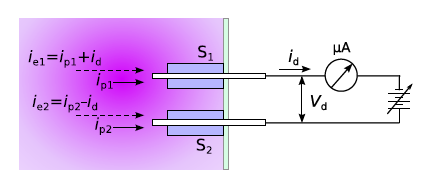
\includegraphics[width=130mm]{schemadvojna.png}
	\caption{Schéma dvojité sondy \cite{navod}.}
	\label{schemadvojna}
\end{figure}


VA charakteristika ideální dvojné rovinné sondy je na
obr. \ref{charakteristikadvojna}. V~bodě $A$, kde platí 
$V_\text{{d}} = 0$ a $i_\text{{d}} = 0$, se obě sondy nachází na
témže plovoucím potenciálu $V_\text{{fl}}$. 

$V_\text{{d}} < 0 $ kolem bodu $B$ je
oblast takzvaného záporného napětí. Platí zde 	
$\sum i_\text{{p}} + \sum i_\text{{e}} = 0$.
Potenciál první ze sond se blíží potenciálu plazmatu,
potenciál druhé sondy bude nižší než plovoucí.

Kolem bodu $C$ platí $V_\text{{d}} \ll 0 $, jedná se tedy
o~oblast VA charakteristiky s~velkým záporným napětím.
První sonda přebírá veškerý tok elektronů, druhá sonda
je silně negativní vzhledem k~potenciálu plazmatu.
Pokud dále vzrůstá $V_\text{{d}}$, dojde k~nasycení
iontového proudu druhé sondy a celkový proud vnějším
okruhem $i_\text{{d}}$ zůstává konstantní.

\begin{figure}[h]
	\centering
	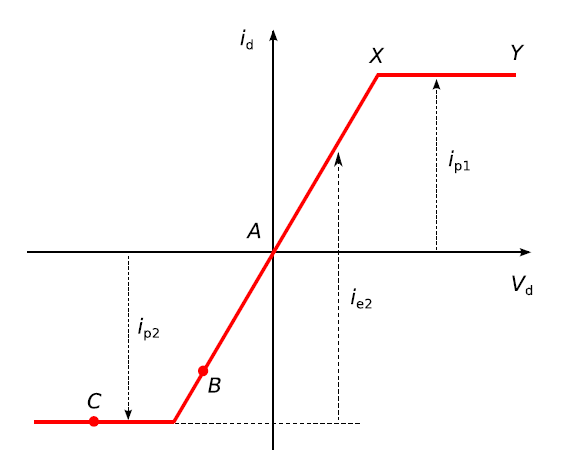
\includegraphics[width=130mm]{charakteristikadvojna.png}
	\caption{Charakteristika ideální dvojné rovinné sondy \cite{navod}.}
	\label{charakteristikadvojna}
\end{figure}
\newpage

\subsection{Výpočet elektronové teploty rezistenční metodou}
Teplotu elektronů můžeme získat ze vztahu

\begin{equation}
	T_\text{{e}} = \frac{e}{k} (G-G^2) R_0 \sum i_\text{{p}}
	\label{T}
\end{equation}
kde $G$ je 
\begin{equation}
	G = \left[ \frac{i_\text{{e2}}}{\sum i_\text{{p}}}\right] 
	\label{G}
\end{equation}
pro $V_\text{{d}} = 0$ a $R_0$ je tzv. ekvivalentní odpor sondy
\begin{equation}
	R_0 = \left[ \frac{\text{d} V_\text{d}} {\text{d}i_\text{d}}
	\right] 
	\label{R}
\end{equation}
opět pro $V_\text{{d}} = 0$. Dále platí
\begin{equation}
	i_\text{{e2}} = |i_\text{{p2}}| + i_\text{{d}}
	\label{ie2}
\end{equation}
\begin{equation}
	\sum i_\text{{p}} = i_\text{{p1}} + i_\text{{p2}}
	\label{sumaip}
\end{equation}

\subsection{Určení elektronové teploty z funkce $\tanh$}
Teplotu elektronů můžeme také určit z graficky
vynesené závislosti
\begin{equation}
	i_\text{{d}} = I_0 \tanh\left( \frac{e V_\text{{d}} }{k T_e} \right) 
	\label{tanh}
\end{equation}

\subsection{Určení koncentrace elektronů}
Koncentraci elektronů za předpokladu $n_\text{{e}}$ = $n_\text{{p}}$
a $T_\text{{e}}$ = $T_\text{{p}}$
lze určit z~rovnice
\begin{equation}
	n_\text{{p}} = \frac{4  i_\text{{p}}}{S e \left\langle v_\text{{p}} 
	\right\rangle }
	\label{ne}
\end{equation}
kde $S$ je plocha sondy a $\left\langle  v_\text{{p}} \right\rangle$ získáme jako
\begin{equation}
	\left\langle v_\text{{p}} \right\rangle = \left( \frac{8 kT_\text{{p}}}{\pi 
	M} \right) 
	\label{vp}
\end{equation}
kde $T_\text{p}$ je teplota iontů a $M$ je hmotnost iontu.

\subsection{Měření a výsledky}
V~našem případě měříme pomocí dvojné symetrické válcové sondy,
obě její části jsou umístěné v~ekvipotenciální ploše plazmatu.
Schéma zapojení sondy je na obr. \ref{zapojenidvojna}. Pracovní
plyn je argon. Provedli jsme tři měření pro proud výbojem  $I_\text{{v}}$ =
55 \si{\milli\ampere} a tlak $p$ = 8--160 \si{\pascal} a jedno
měření s~odlišným proudem $I_\text{{v}}$ =
30 \si{\milli\ampere} při tlaku $p$ = 160 \si{\pascal}.

\begin{figure}[h]
	\centering
	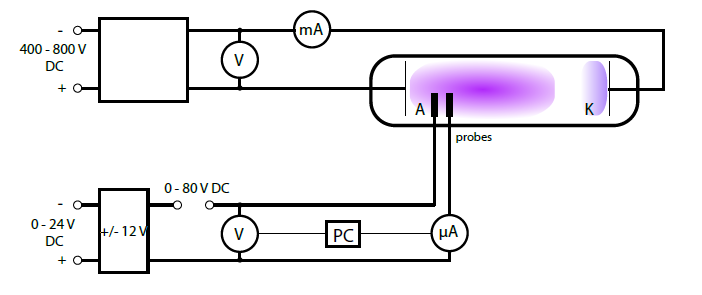
\includegraphics[width=130mm]{zapojenidvojna.png}
	\caption{Schéma zapojení měřící aparatury \cite{navod}.}
	\label{zapojenidvojna}
\end{figure}

\begin{figure}[h]
	\centering
	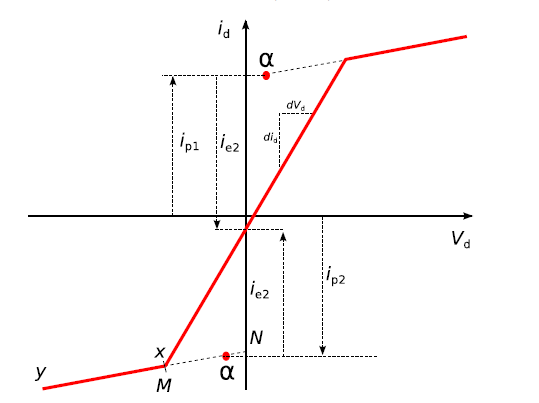
\includegraphics[width=130mm]{VAmerenidvojna.png}
	\caption{Vyhodnocení VA charakteristiky dvojné sondy \cite{navod}.}
	\label{VAmerenidvojna}
\end{figure}
Vyhodnocení dat provedeme podle obr. \ref{VAmerenidvojna}.
Všechny tři lineární oblasti charakteristiky proložíme přímkou.
Poté určíme bod $\alpha$, který se nachází ve vzdálenosti
$\frac{1}{5}MN$ od osy $y$. V~bodě~$\alpha$ lze určit proudy
$i_\text{{p1}}$ a $i_\text{{p2}}$. Proud $i_\text{{d}}$
získáme jako průsečík VA charakteristiky s~$y$~osou v~bodě
$x$~=~0. Grafy charakteristik, ze kterých odečítáme výše
zmíněné veličiny, jsou na obr. \ref{dvojna1} až \ref{dvojna4}.
$R_0$ určíme ze směrnice přímky, kterou jsme proložili
střední strmou část charakteristiky, viz rovnice \eqref{R}.
Zbylé veličiny, tedy $i_\text{{e2}}$ a $G$ spočítáme z~rovnic
\eqref{ie2}, \eqref{sumaip} a \eqref{G}. Plochu sondy $S$
jsme spočítali pomocí odhadnutých rozměrů ze vztahu \eqref{S},
kde její délka je $l = 8$ \si{\milli\meter} a její poloměr
$r = 0,05$ \si{\milli\meter}. Tloušťka stěnové
vrstvy je odhadem $d = 1$ \si{\centi\meter}.

\begin{equation}
	S = \pi (r+d)^2 + 2\pi (r+d) l = 8,22\cdot 10^{-4} \si{\meter\squared}
	\label{S}
\end{equation}

Pak již můžeme
spočítat teplotu elektronů z~rovnice \eqref{T} a koncentraci
elektronů z~\eqref{ne}, výsledky jsou v~tabulce~\ref{tab1}.
Vidíme, že s~rostoucím tlakem roste koncentrace elektronů.
Teplota elektronů nevykazuje žádný trend. Při snížení proudu
výboje za konstantního tlaku dojde ke snížení teploty i~koncentrace
elektronů.
\newpage
Teplotu určíme i druhým způsobem, tedy pomocí rovnice
\eqref{tanh}. Proložení charakteristik funkcí $\tanh$
je vidět........XXXXXXXXXXXXXXX
a dopočítaná koncentrace elektronů ze vztahu \eqref{ne}
je v tabulce

\newpage
\begin{figure}[h!]
	\centering
	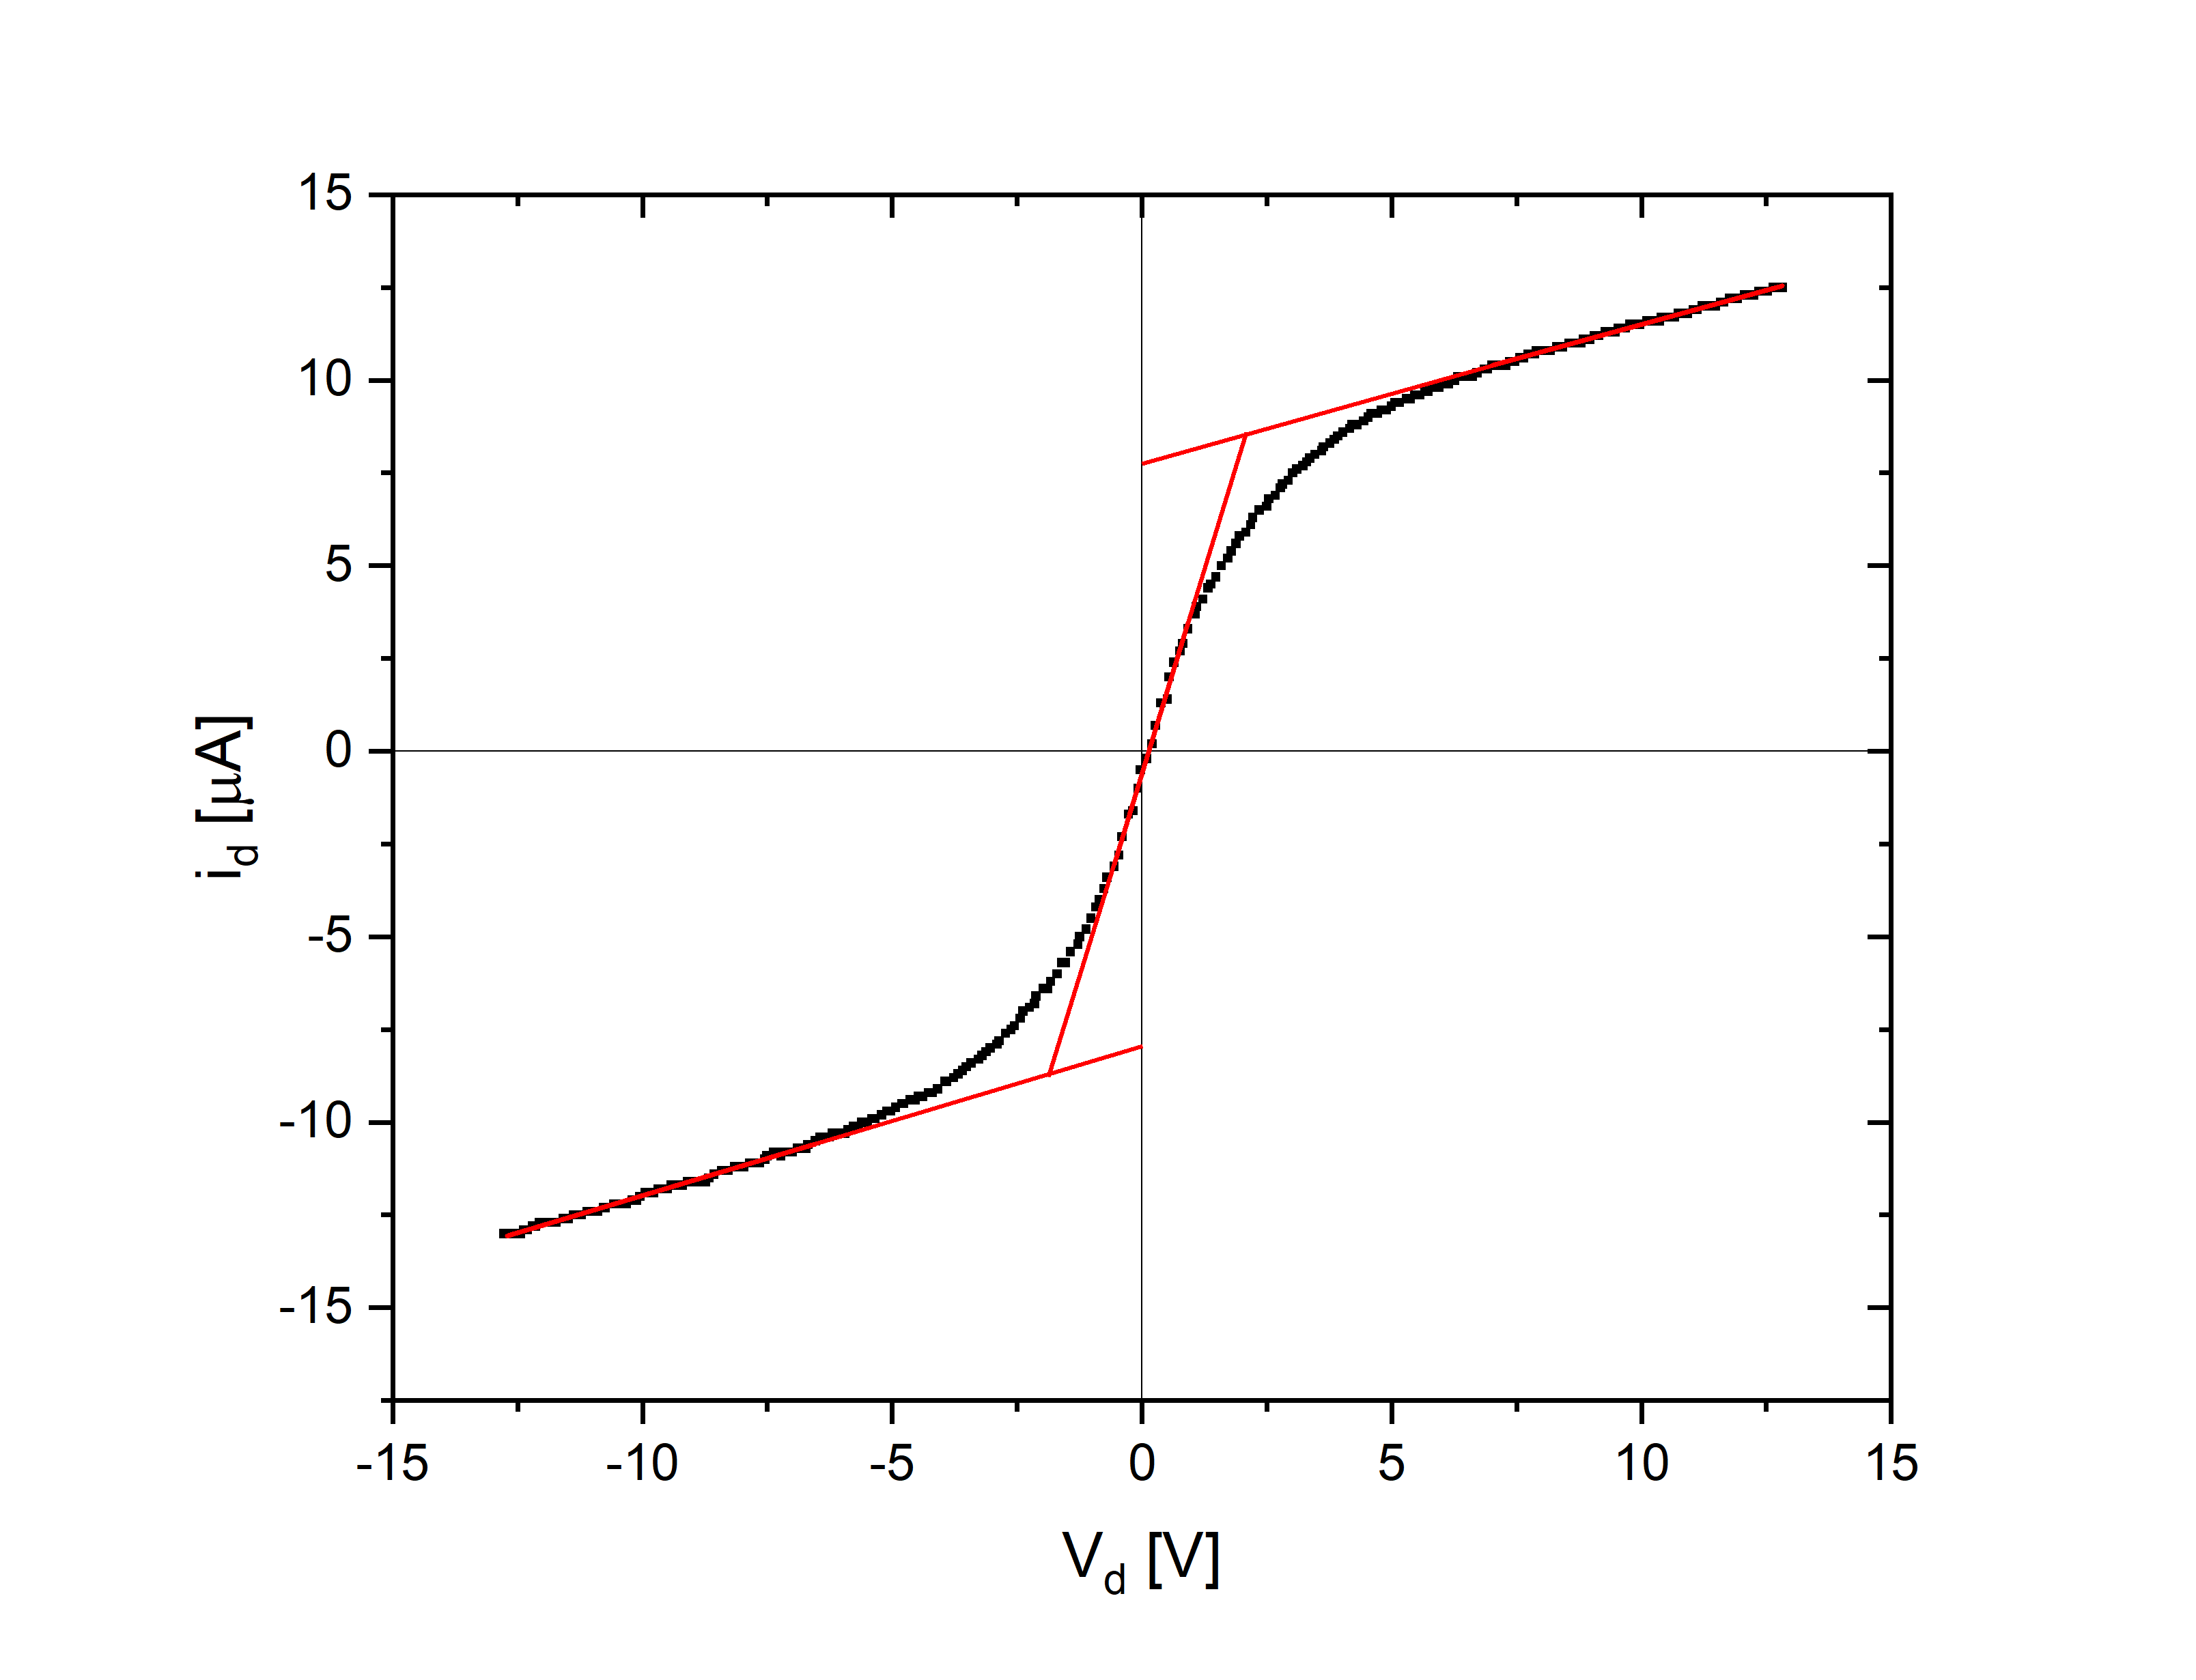
\includegraphics[width=130mm]{dvojna1.png}
	\caption{VA charakteristika za podmínek $p$ = 8 \si{\pascal}, $I_\text{{v}}$ = 55 \si{\milli\ampere}.}
	\label{dvojna1}
\end{figure}

\begin{figure}[h!]
	\centering
	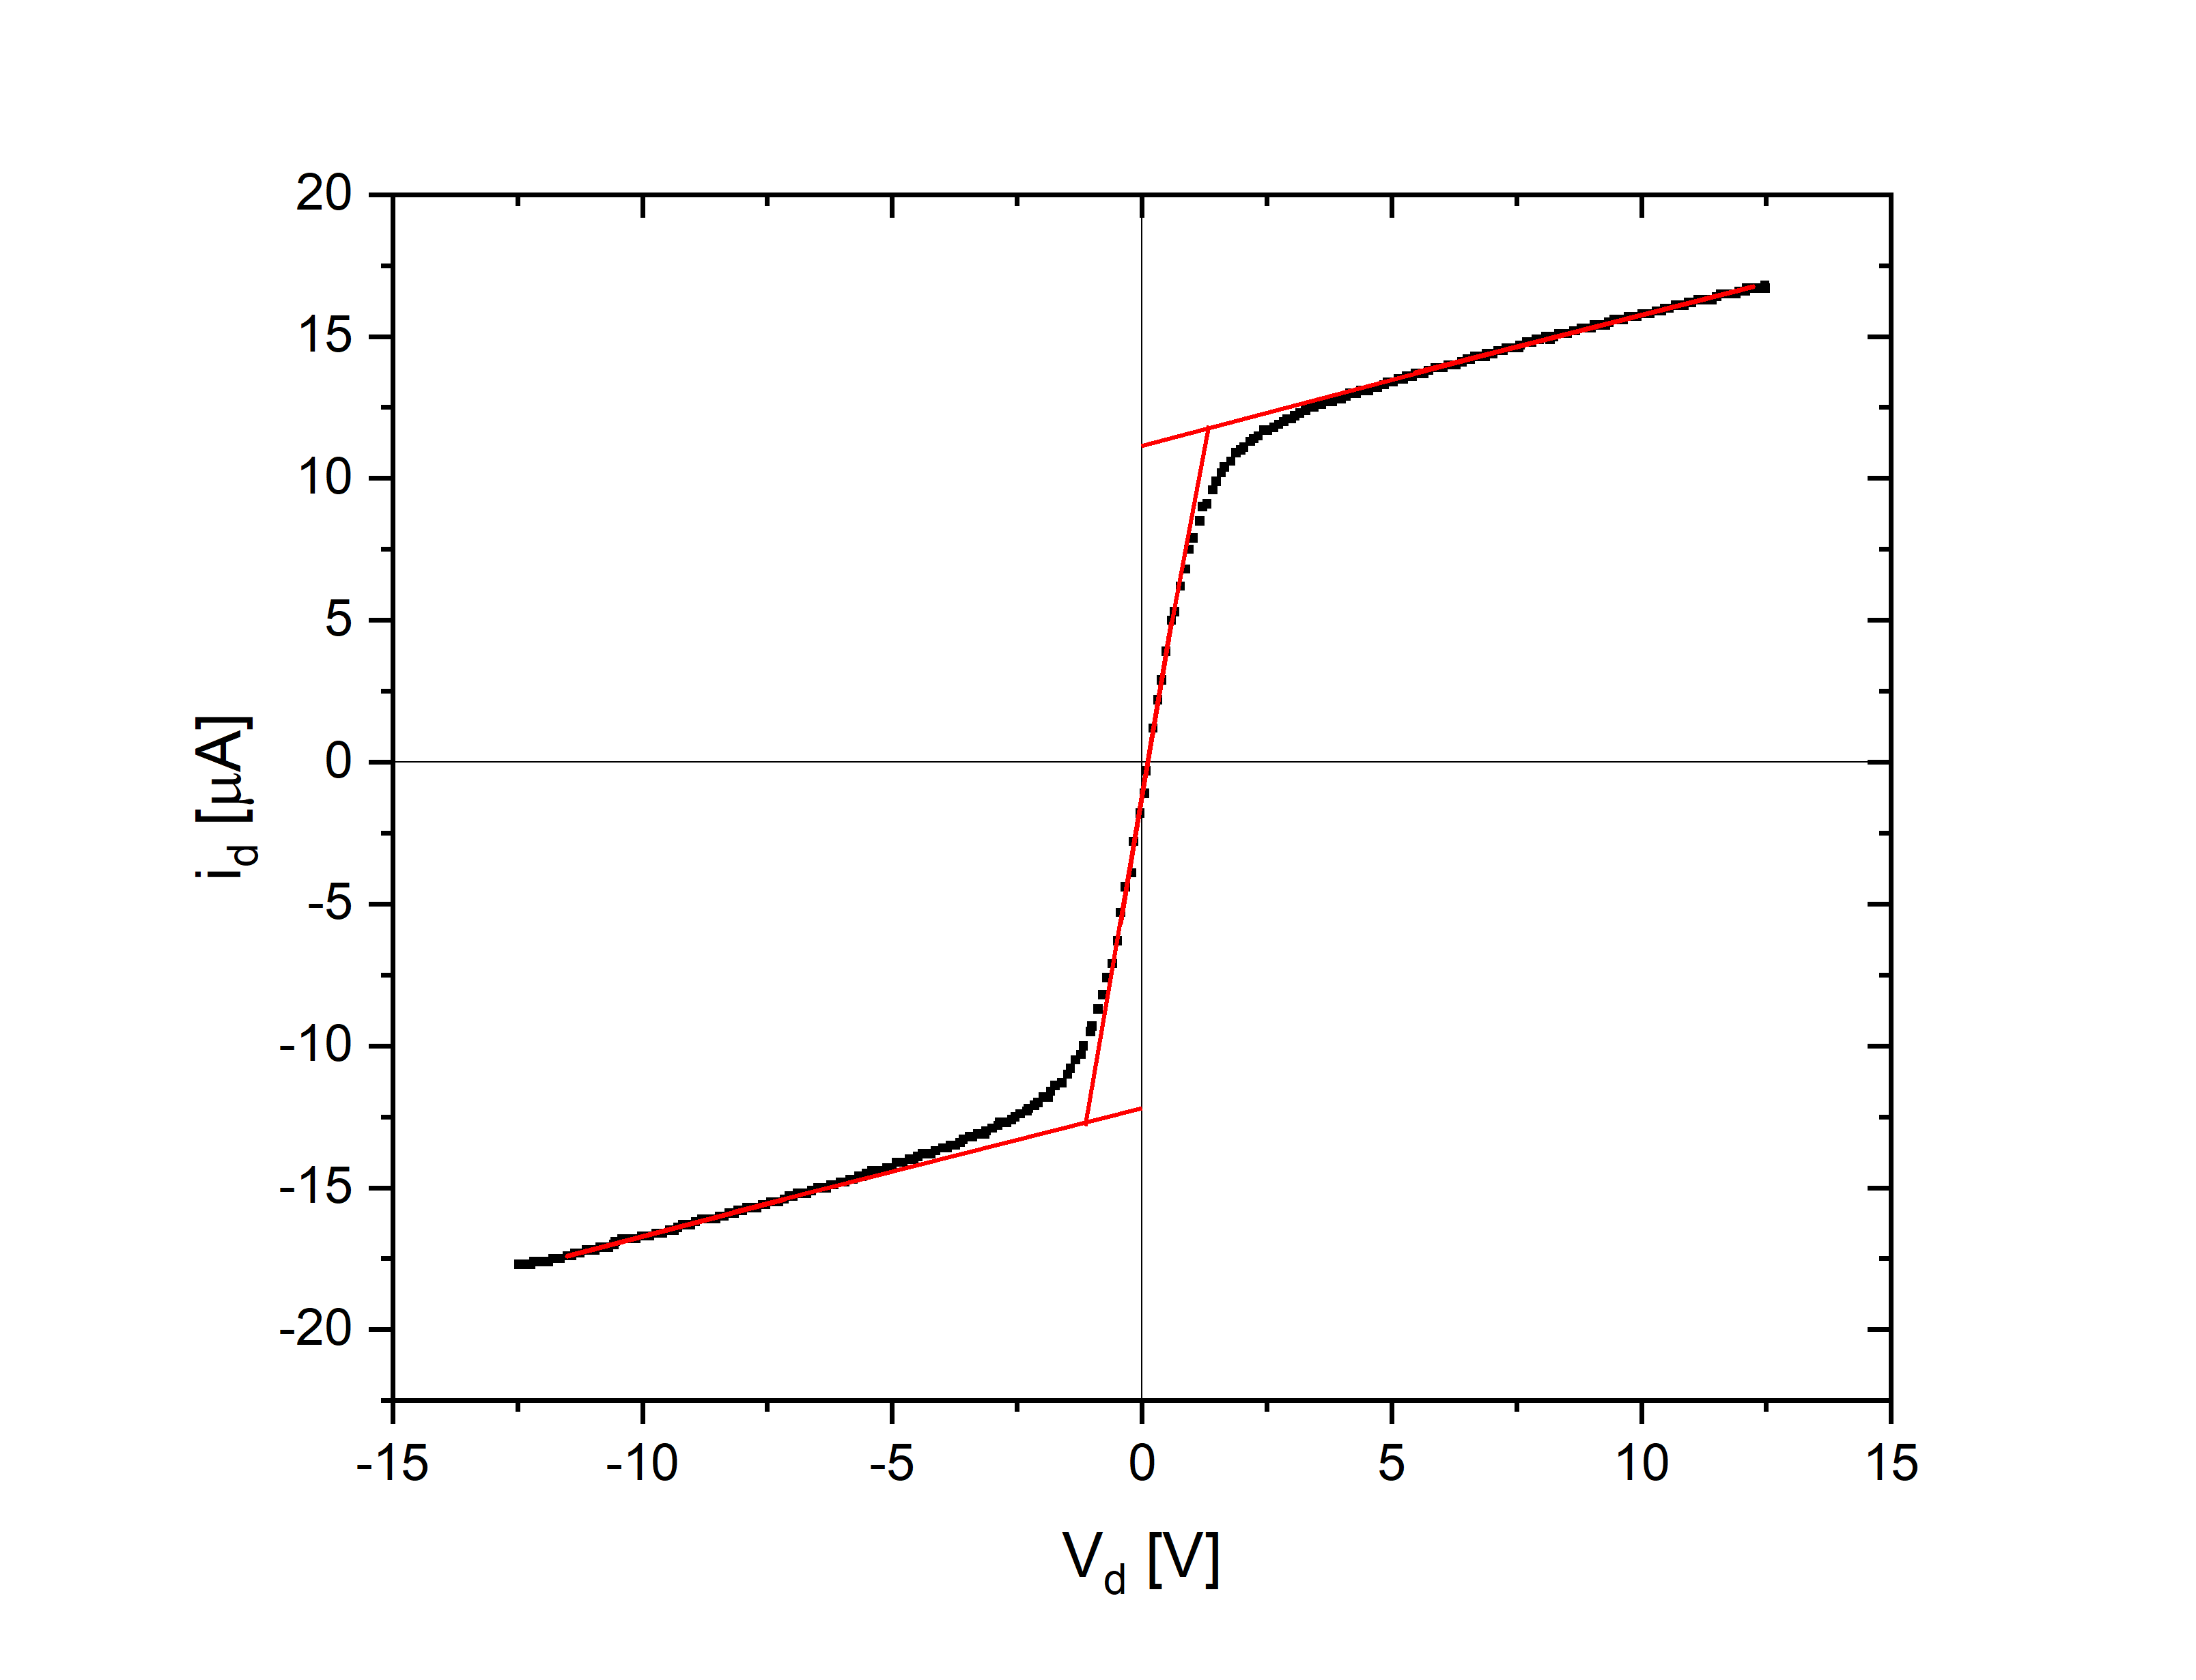
\includegraphics[width=130mm]{dvojna2.png}
	\caption{VA charakteristika za podmínek $p$ = 32 \si{\pascal}, $I_\text{{v}}$ = 55 \si{\milli\ampere}.}
	\label{dvojna2}
\end{figure}

\begin{figure}[h!]
	\centering
	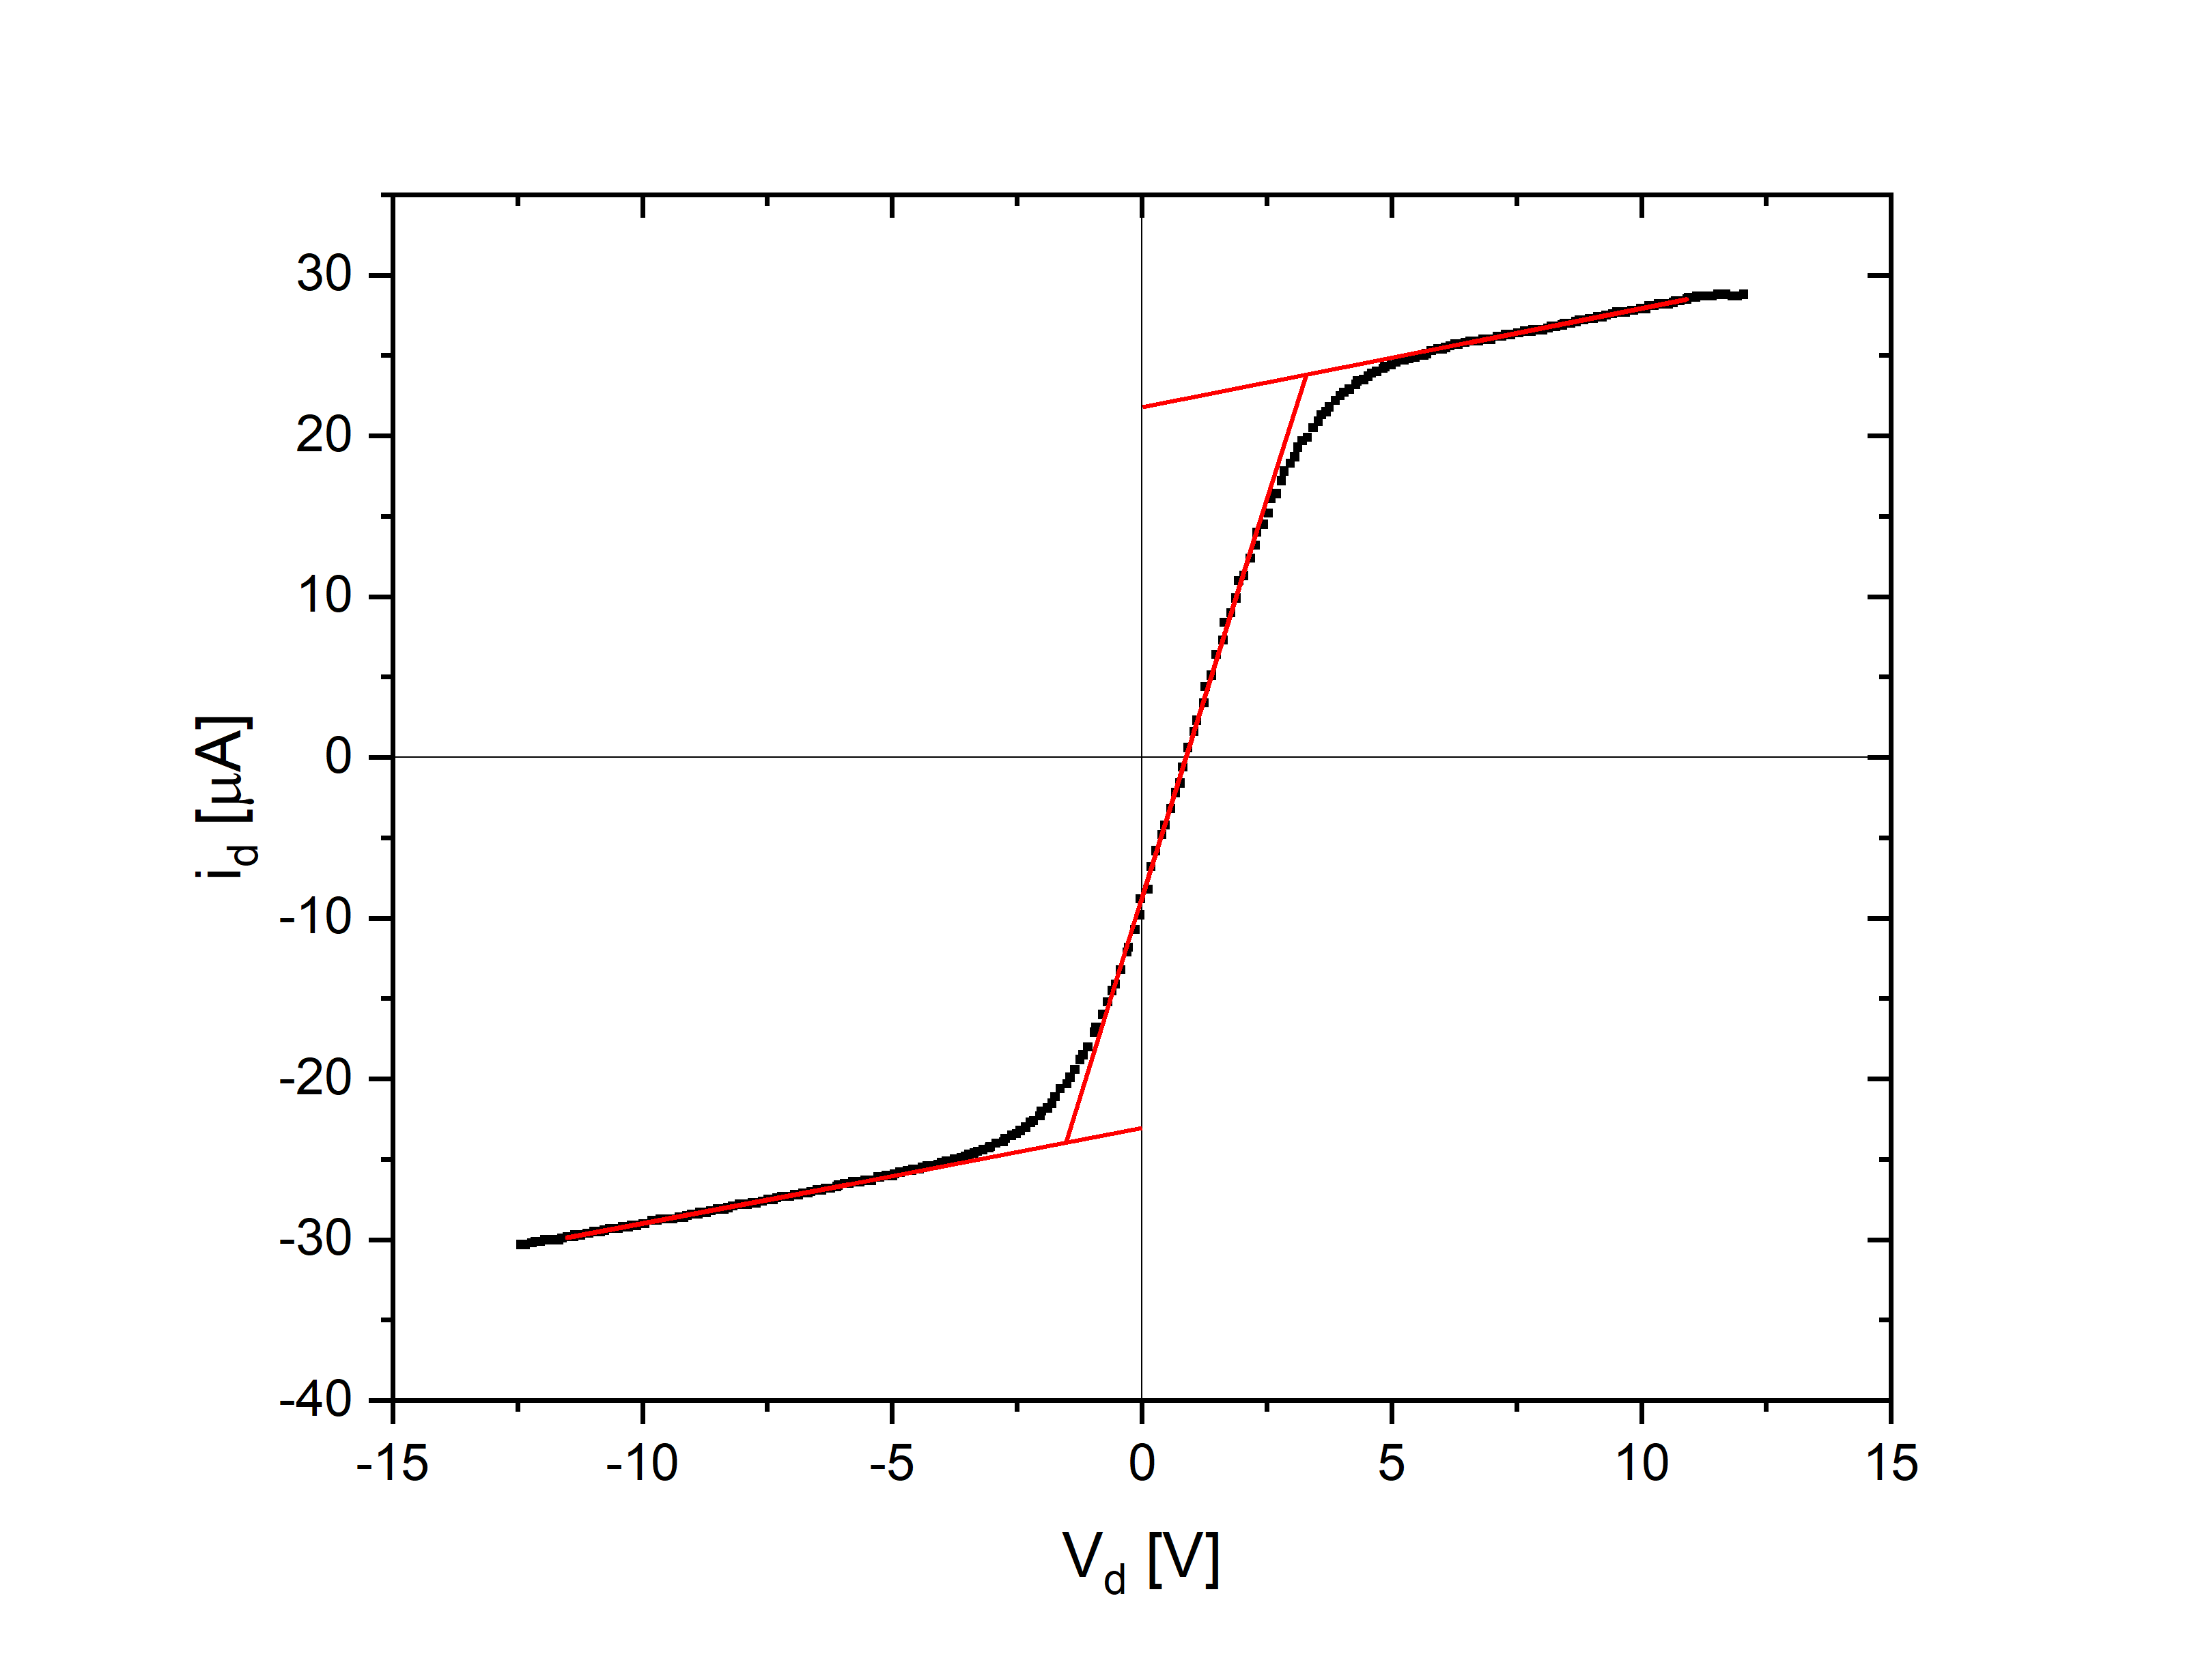
\includegraphics[width=130mm]{dvojna3.png}
	\caption{VA charakteristika za podmínek $p$ = 160 \si{\pascal}, $I_\text{{v}}$ = 55 \si{\milli\ampere}.}
	\label{dvojna3}
\end{figure}

\begin{figure}[h!]
	\centering
	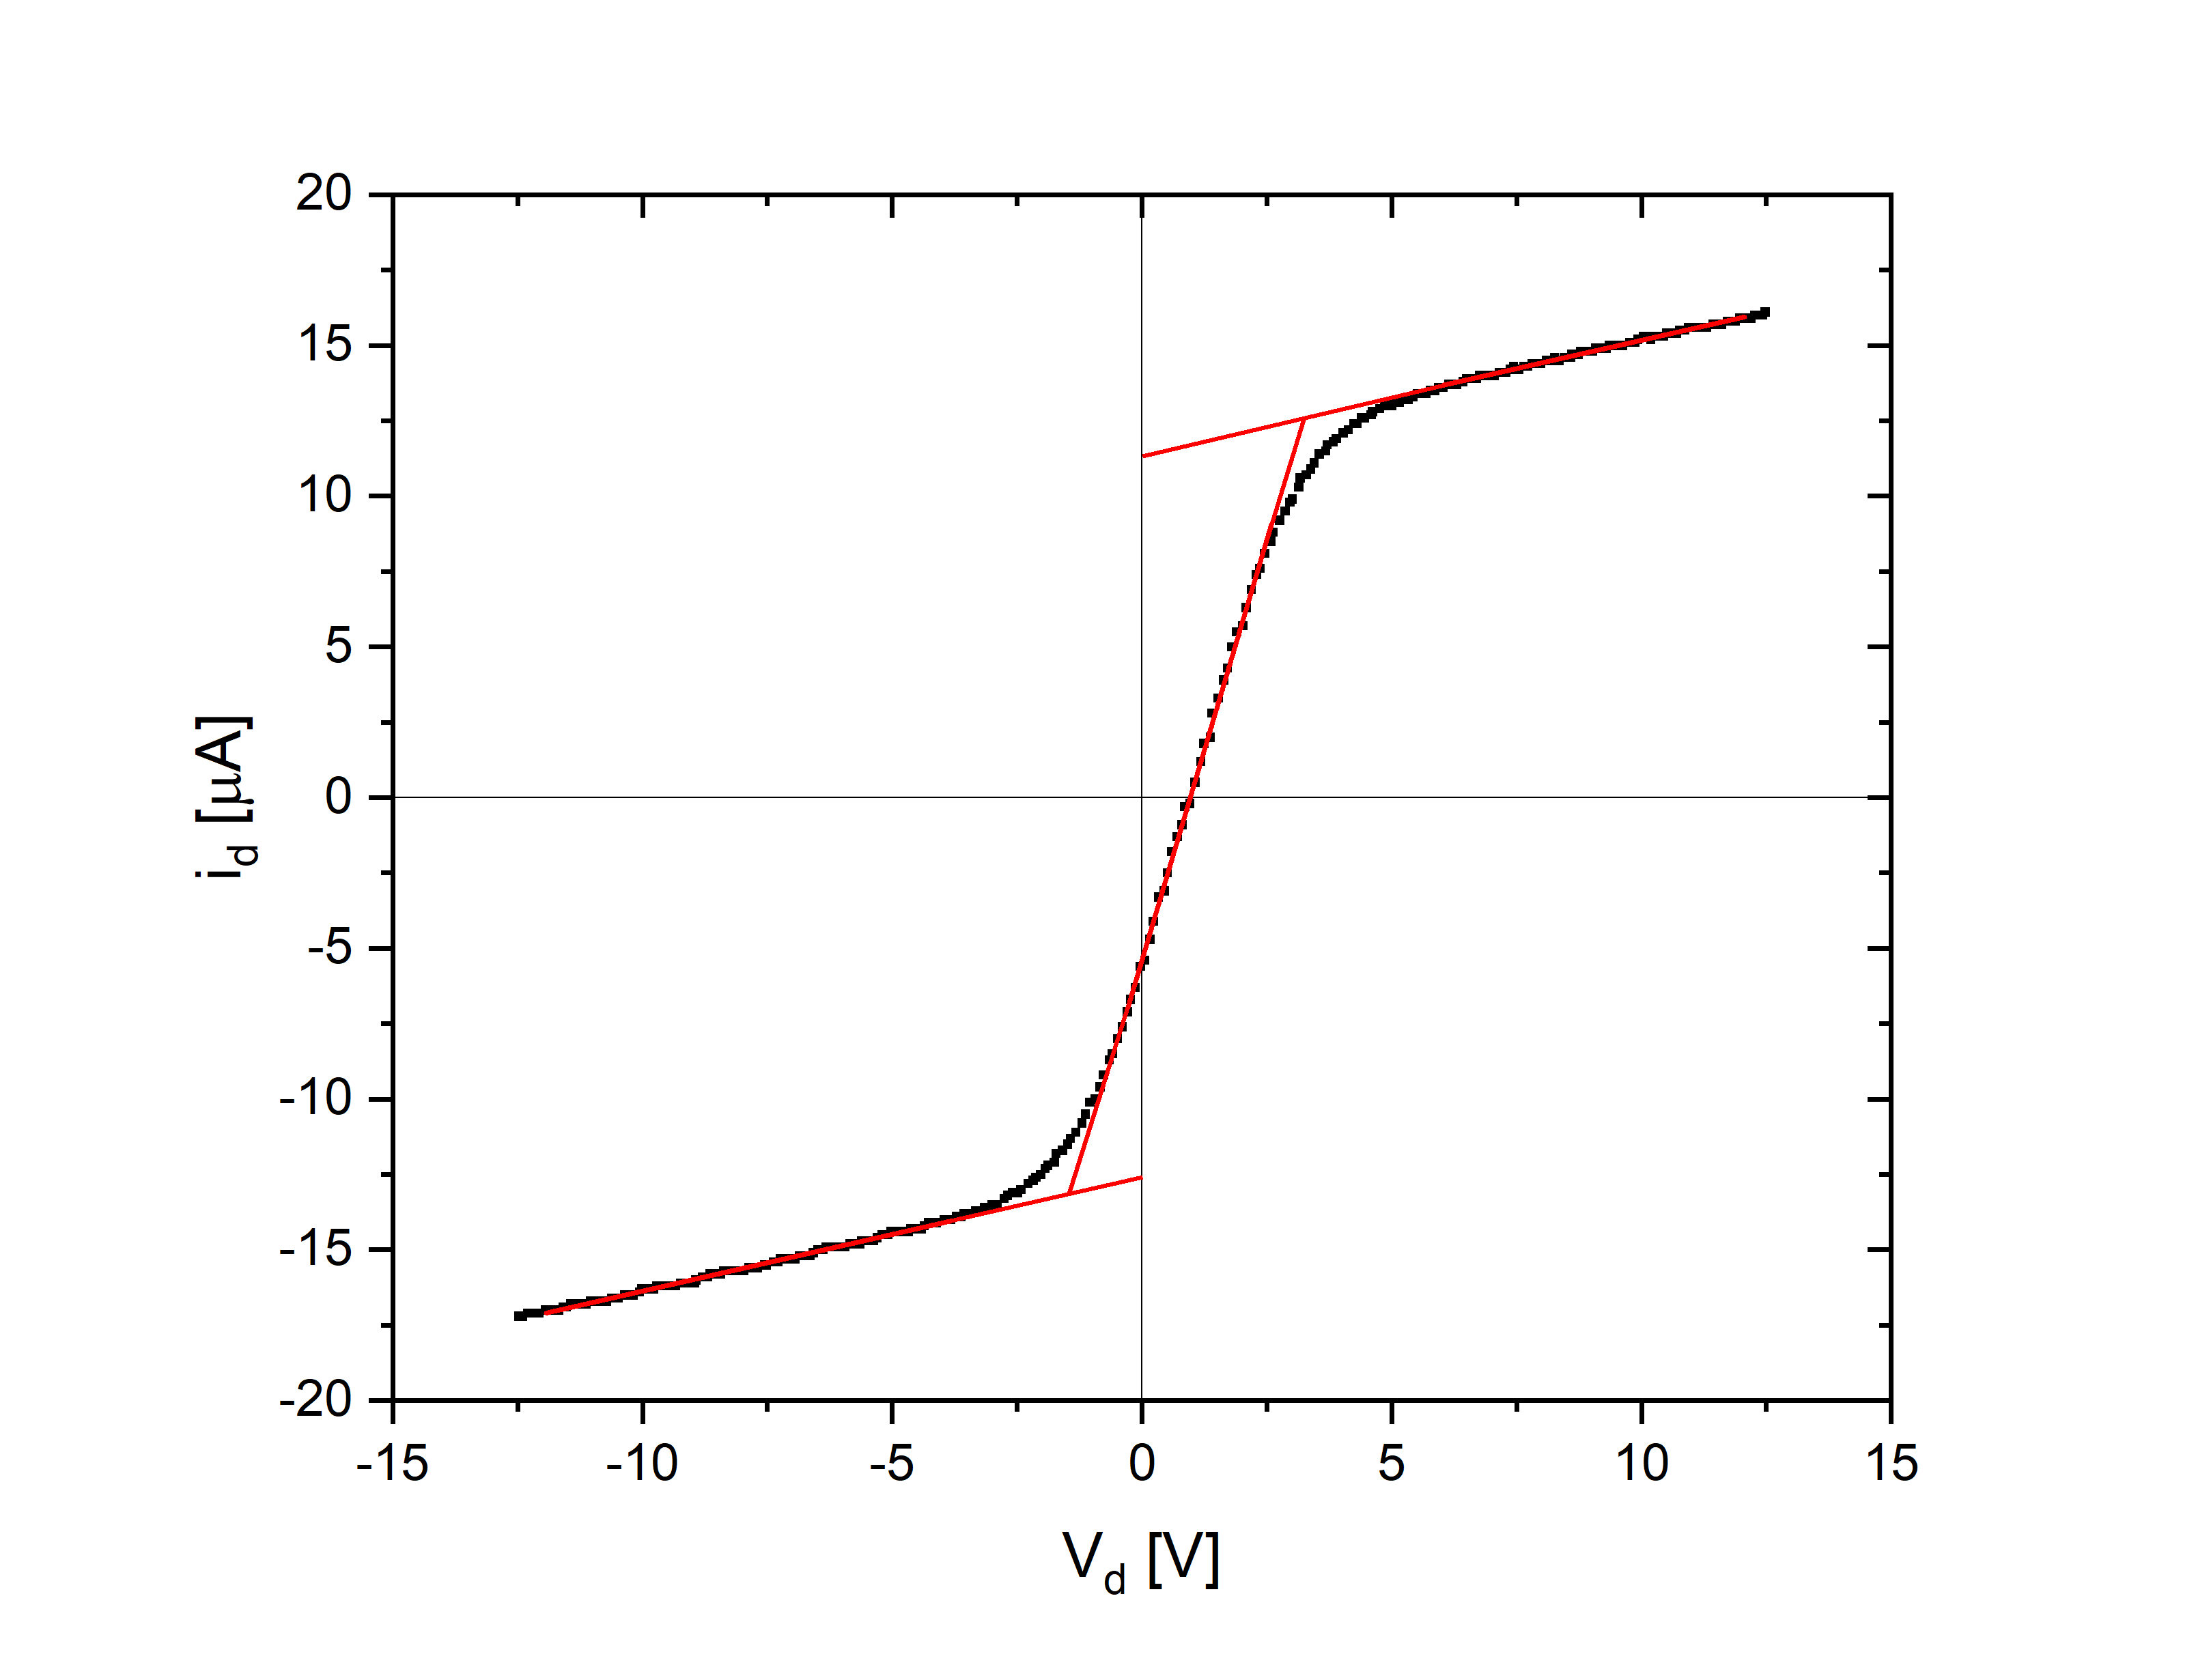
\includegraphics[width=130mm]{dvojna4.png}
	\caption{VA charakteristika za podmínek $p$ = 160 \si{\pascal}, $I_\text{{v}}$ = 30 \si{\milli\ampere}.}
	\label{dvojna4}
\end{figure}

\newpage
\begin{center}
	\begin{table}[h!]
		\centering
		\caption{Teploty a koncentrace elektronů.}
		\label{tab1}
		\begin{tabular}{|c|c|c|c|c|c|} \hline
			\multicolumn{3}{|c|}{$I_\text{v}$ = 55 \si{\milli\ampere}}& \multicolumn{3}{c|}{$p$ = 160 [\si{\pascal}] }  \\ \hline
			$p$ [\si{\pascal}] & $T_\text{e}$ [\si{\electronvolt}]  & $n_\text{e}$ [$10^{14}$ \si{\per\meter\cubed}]& $I_\text{v}$ [\si{\milli\ampere}] & $T_\text{e}$ [\si{\electronvolt}] & $n_\text{e}$  [$10^{14}$ \si{\per\meter\cubed}]\\ \hline
			8 & 0,91 & 1,68 & 30 & 0,92 & 4,87\\ \hline
			32 & 0,57 & 6,04 &  &  &  \\ \hline
			160 & 1,00 & 8,96 &  &  &  \\ \hline
			
		\end{tabular}
	\end{table}
\end{center}

\newpage
\section{Závěr}
V~této úloze jsme se seznámili s~měřením důležitých veličin plazmatu pomocí dvojné sondy.
Z~naměřených charakteristik za různých podmínek se nám povedlo určit teplotu
elektronů~$T_\text{e}$ a jejich koncentraci $n_\text{e}$. Teplota elektronů s~rostoucím tlakem
nevykazuje žádný trend, koncentrace elektronů však roste. Za sníženého proudu výbojem
při udržování konstantního tlaku klesla teplota i koncentrace elektronů.

\newpage
\begin{thebibliography}{10}
	\bibitem{navod} Návod k praktiku: \textit{Studium kladného sloupce doutnavého výboje pomocí elektrostatických sond: dvojná sonda.}
	
\end{thebibliography}


\end{document}
